\documentclass[border=15pt]{standalone}
\usepackage{tikz}
\usepackage{amsmath}
\usepackage{amssymb}
\usetikzlibrary{positioning,shapes.geometric,arrows.meta,calc,shadows.blur,backgrounds,fit}

\begin{document}
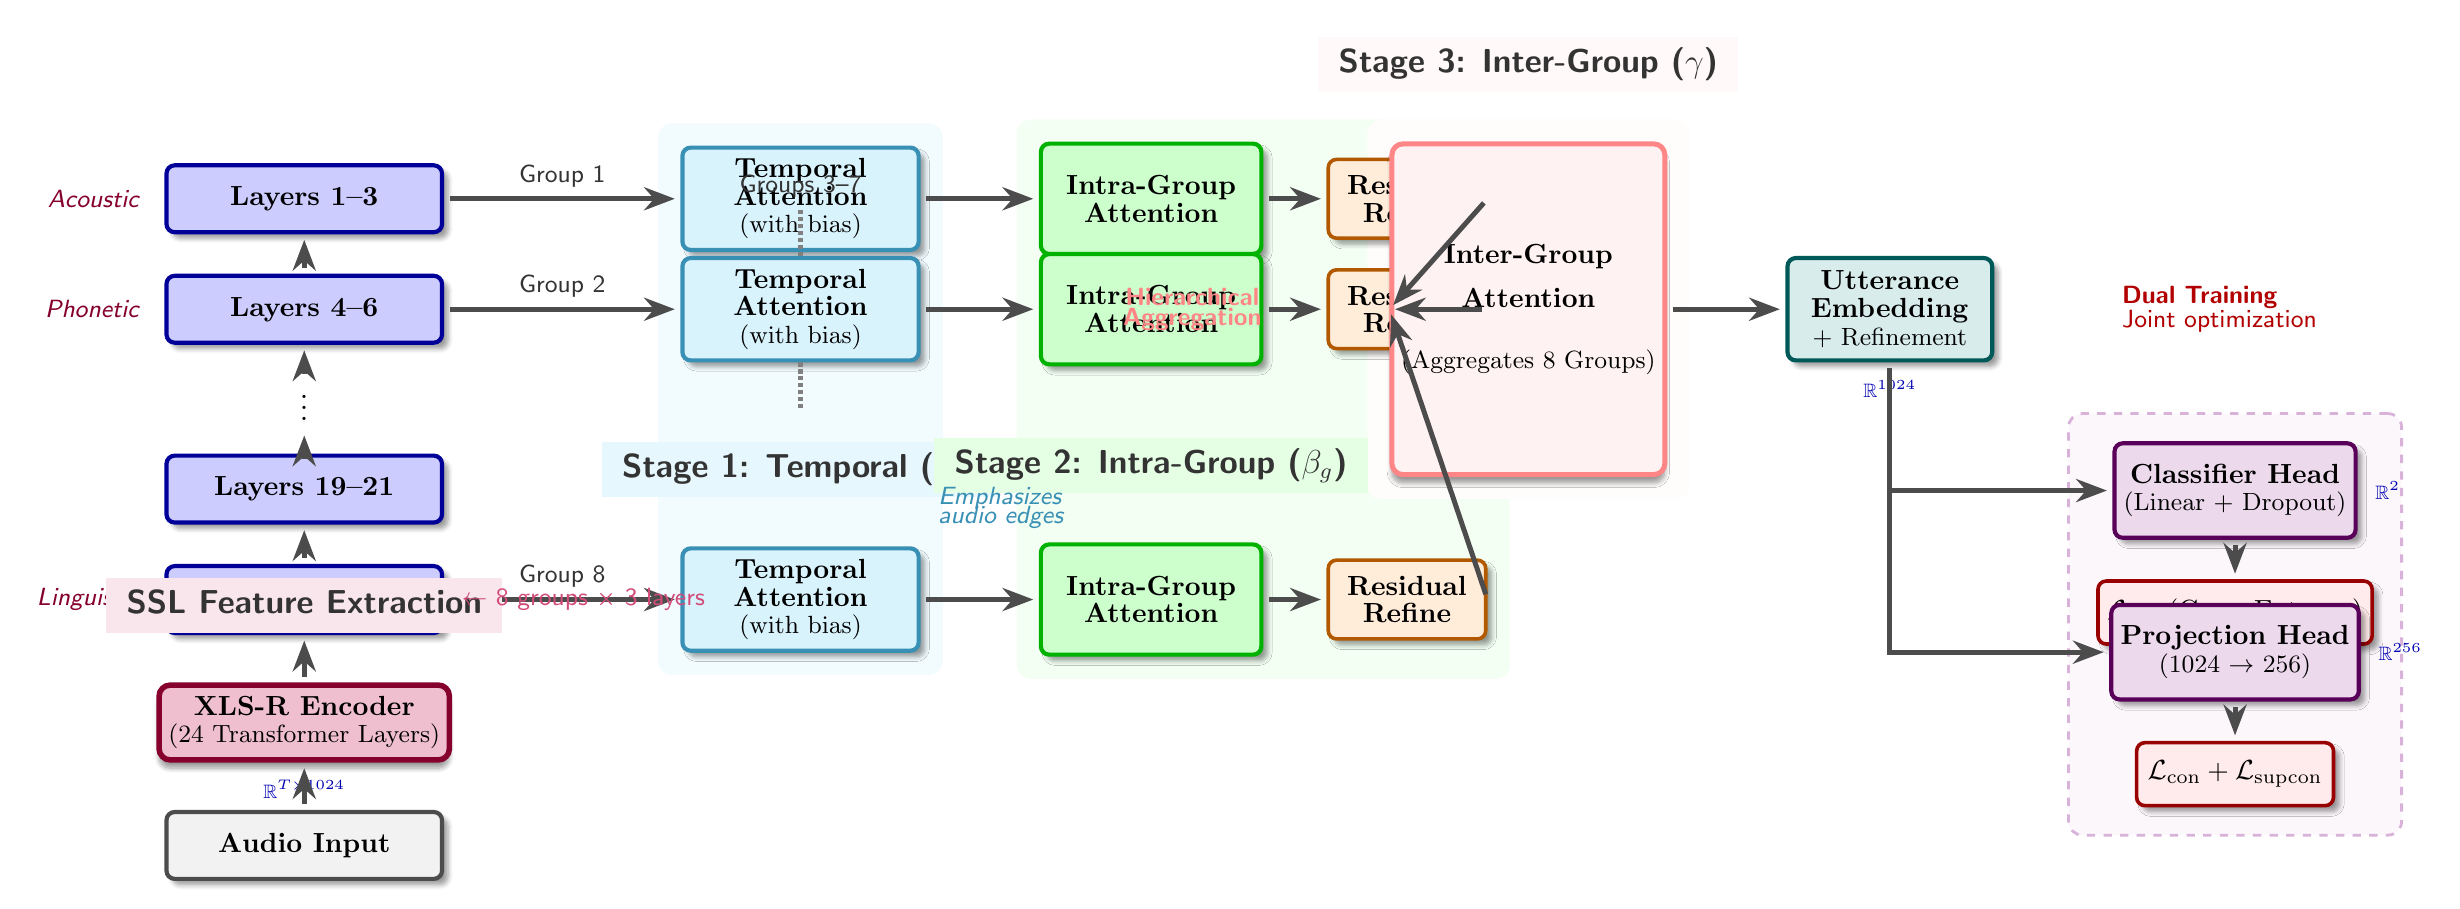
\begin{tikzpicture}[
    node distance=0.8cm,
    % Modern color palette with gradients
    layer/.style={rectangle, draw=blue!60!black, line width=1.5pt, minimum width=3.5cm, minimum height=0.85cm, 
                  align=center, fill=blue!20, rounded corners=3pt, blur shadow={shadow blur steps=5}},
    xlsr/.style={rectangle, draw=purple!70!black, line width=2pt, minimum width=3.5cm, minimum height=0.95cm, 
                align=center, fill=purple!25, rounded corners=4pt, blur shadow={shadow blur steps=8, shadow xshift=0pt, shadow yshift=-3pt}},
    temporal/.style={rectangle, draw=cyan!70!black, line width=1.5pt, minimum width=3cm, minimum height=1.3cm, 
                    align=center, fill=cyan!15, rounded corners=3pt, blur shadow={shadow blur steps=5}},
    intra/.style={rectangle, draw=green!70!black, line width=1.5pt, minimum width=2.8cm, minimum height=1.4cm, 
                 align=center, fill=green!20, rounded corners=3pt, blur shadow={shadow blur steps=5}},
    refine/.style={rectangle, draw=orange!70!black, line width=1.3pt, minimum width=2cm, minimum height=1cm, 
                  align=center, fill=orange!15, rounded corners=3pt, blur shadow={shadow blur steps=5}},
    inter/.style={rectangle, draw=pink!70!red, line width=1.8pt, minimum width=2.8cm, minimum height=4.2cm, 
                 align=center, fill=pink!20, rounded corners=4pt, blur shadow={shadow blur steps=8, shadow xshift=0pt, shadow yshift=-3pt}},
    utt/.style={rectangle, draw=teal!70!black, line width=1.5pt, minimum width=2.6cm, minimum height=1.3cm, 
               align=center, fill=teal!15, rounded corners=3pt, blur shadow={shadow blur steps=5}},
    head/.style={rectangle, draw=violet!70!black, line width=1.5pt, minimum width=2.5cm, minimum height=1.2cm, 
                align=center, fill=violet!15, rounded corners=3pt, blur shadow={shadow blur steps=5}},
    loss/.style={rectangle, draw=red!60!black, line width=1.3pt, minimum width=2.5cm, minimum height=0.8cm, 
                align=center, fill=red!8, rounded corners=3pt, blur shadow={shadow blur steps=5}},
    input/.style={rectangle, draw=gray!60!black, line width=1.5pt, minimum width=3.5cm, minimum height=0.85cm, 
                 align=center, fill=gray!10, rounded corners=3pt, blur shadow={shadow blur steps=5}},
    arrow/.style={-Stealth, line width=1.8pt, draw=black!70, shorten >=2pt, shorten <=2pt},
    dotted_arrow/.style={densely dotted, line width=1.5pt, draw=black!50},
    label/.style={font=\small\sffamily, text=black!80},
    dimension/.style={font=\scriptsize\ttfamily, text=blue!70!black},
    stage_label/.style={font=\large\bfseries\sffamily, text=black!80},
    semantic_label/.style={font=\small\itshape\sffamily, text=purple!70!black}
]

% ========== INPUT LAYER ==========
\node[input] (input) {\textbf{Audio Input}};

% ========== XLS-R ENCODER ==========
\node[xlsr, above=0.6cm of input] (xlsr) {\textbf{XLS-R Encoder}\\[-2pt]\small(24 Transformer Layers)};
\node[dimension, below=0.1cm of xlsr] {$\mathbb{R}^{T \times 1024}$};

% ========== LAYER GROUPS ==========
\node[layer, above=0.6cm of xlsr] (g8) {\textbf{Layers 22--24}};
\node[semantic_label, left=0.2cm of g8] (sem_high) {Linguistic};

\node[layer, above=0.5cm of g8] (g7) {\textbf{Layers 19--21}};

\node[above=0.3cm of g7, font=\large] (dots1) {$\vdots$};

\node[layer, above=0.3cm of dots1] (g2) {\textbf{Layers 4--6}};
\node[semantic_label, left=0.2cm of g2] (sem_mid) {Phonetic};

\node[layer, above=0.5cm of g2] (g1) {\textbf{Layers 1--3}};
\node[semantic_label, left=0.2cm of g1] (sem_low) {Acoustic};

% ========== STAGE 1: TEMPORAL ATTENTION ==========
\node[temporal, right=3cm of g1] (temp_low) {\textbf{Temporal}\\[-2pt]\textbf{Attention}\\[-2pt]\small(with bias)};
\node[dimension, below=0.1cm of temp_low] {$\mathbb{R}^{1024}$};

\node[temporal, right=3cm of g2] (temp_mid) {\textbf{Temporal}\\[-2pt]\textbf{Attention}\\[-2pt]\small(with bias)};

\node[temporal, right=3cm of g8] (temp_high) {\textbf{Temporal}\\[-2pt]\textbf{Attention}\\[-2pt]\small(with bias)};

% ========== STAGE 2: INTRA-GROUP ATTENTION ==========
\node[intra, right=1.5cm of temp_low] (intra_low) {\textbf{Intra-Group}\\[-2pt]\textbf{Attention}};
\node[refine, right=0.8cm of intra_low] (ref_low) {\textbf{Residual}\\[-2pt]\textbf{Refine}};

\node[intra, right=1.5cm of temp_mid] (intra_mid) {\textbf{Intra-Group}\\[-2pt]\textbf{Attention}};
\node[refine, right=0.8cm of intra_mid] (ref_mid) {\textbf{Residual}\\[-2pt]\textbf{Refine}};

\node[intra, right=1.5cm of temp_high] (intra_high) {\textbf{Intra-Group}\\[-2pt]\textbf{Attention}};
\node[refine, right=0.8cm of intra_high] (ref_high) {\textbf{Residual}\\[-2pt]\textbf{Refine}};

% ========== STAGE 3: INTER-GROUP ATTENTION ==========
\node[inter, right=1.6cm of intra_mid] (inter) {\textbf{Inter-Group}\\[4pt]\textbf{Attention}\\[10pt]\small(Aggregates 8 Groups)};

% ========== UTTERANCE EMBEDDING ==========
\node[utt, right=1.5cm of inter] (utt_emb) {\textbf{Utterance}\\[-2pt]\textbf{Embedding}\\[-2pt]\small+ Refinement};
\node[dimension, below=0.1cm of utt_emb] {$\mathbb{R}^{1024}$};

% ========== DUAL HEADS ==========
\node[head, below right=1cm and 1.5cm of utt_emb] (classifier) {\textbf{Classifier Head}\\[-2pt]\small(Linear + Dropout)};
\node[dimension, right=0.1cm of classifier] {$\mathbb{R}^{2}$};

\node[loss, below=0.5cm of classifier] (ce_loss) {$\mathcal{L}_{\text{CE}}$ (Cross-Entropy)};

\node[head, below=0.8cm of classifier] (projection) {\textbf{Projection Head}\\[-2pt]\small(1024 $\to$ 256)};
\node[dimension, right=0.1cm of projection] {$\mathbb{R}^{256}$};

\node[loss, below=0.5cm of projection] (con_loss) {$\mathcal{L}_{\text{con}} + \mathcal{L}_{\text{supcon}}$};

% ========== ARROWS: INPUT TO ENCODER ==========
\draw[arrow] (input) -- (xlsr);

% ========== ARROWS: ENCODER TO GROUPS ==========
\draw[arrow] (xlsr) -- (g8);
\draw[arrow] (g8) -- (g7);
\draw[arrow] (g7) -- (dots1);
\draw[arrow] (dots1) -- (g2);
\draw[arrow] (g2) -- (g1);

% ========== ARROWS: GROUPS TO TEMPORAL ==========
\draw[arrow] (g1.east) -- node[above, label] {\small Group 1} (temp_low.west);
\draw[arrow] (g2.east) -- node[above, label] {\small Group 2} (temp_mid.west);
\draw[arrow] (g8.east) -- node[above, label] {\small Group 8} (temp_high.west);

% Groups 3-7 dotted connection
\draw[dotted_arrow] (temp_mid.north) -- ++(0,0.6) node[above, label] {\small Groups 3--7};
\draw[dotted_arrow] (temp_mid.south) -- ++(0,-0.6);

% ========== ARROWS: TEMPORAL TO INTRA ==========
\draw[arrow] (temp_low) -- (intra_low);
\draw[arrow] (temp_mid) -- (intra_mid);
\draw[arrow] (temp_high) -- (intra_high);

% ========== ARROWS: INTRA TO REFINE ==========
\draw[arrow] (intra_low) -- (ref_low);
\draw[arrow] (intra_mid) -- (ref_mid);
\draw[arrow] (intra_high) -- (ref_high);

% ========== ARROWS: REFINE TO INTER ==========
\draw[arrow] (ref_low.east) -- (inter.west);
\draw[arrow] (ref_mid.east) -- (inter.west);
\draw[arrow] (ref_high.east) -- (inter.west);

% ========== ARROW: INTER TO UTTERANCE ==========
\draw[arrow] (inter) -- (utt_emb);

% ========== ARROWS: UTTERANCE TO HEADS ==========
\draw[arrow] (utt_emb.south) |- (classifier.west);
\draw[arrow] (utt_emb.south) |- (projection.west);

% ========== ARROWS: HEADS TO LOSSES ==========
\draw[arrow] (classifier) -- (ce_loss);
\draw[arrow] (projection) -- (con_loss);

% ========== STAGE LABELS ==========
\node[stage_label, above=0.5cm of xlsr] {\colorbox{purple!10}{\strut\ SSL Feature Extraction\ }};
\node[stage_label, above=0.5cm of temp_high] {\colorbox{cyan!10}{\strut\ Stage 1: Temporal ($\alpha_t$)\ }};
\node[stage_label, above=0.5cm of intra_high] {\colorbox{green!10}{\strut\ Stage 2: Intra-Group ($\beta_g$)\ }};
\node[stage_label, above=0.5cm of inter] {\colorbox{pink!10}{\strut\ Stage 3: Inter-Group ($\gamma$)\ }};

% ========== GROUP SIZE ANNOTATION ==========
\node[label, right=0.1cm of g8, text=purple!70] {$\leftarrow$ 8 groups × 3 layers};

% ========== DUAL OBJECTIVE ANNOTATION ==========
\node[label, right=1.5cm of utt_emb, align=left, text=red!70!black] {
    \textbf{Dual Training}\\[-2pt]
    \small Joint optimization
};

% ========== KEY INNOVATION CALLOUTS ==========
% Temporal bias callout
\node[label, above right=0.1cm and 0.1cm of temp_high, text=cyan!70!black, align=left] {
    \textit{Emphasizes}\\[-4pt]
    \textit{audio edges}
};

% Hierarchical callout
\node[label, left=1.5cm of inter, text=pink!70!red, align=center] {
    \textbf{Hierarchical}\\[-4pt]
    \textbf{Aggregation}
};

% ========== BACKGROUND BOXES FOR STAGES ==========
\begin{scope}[on background layer]
    % Stage 1 background
    \node[fit=(temp_low)(temp_mid)(temp_high), fill=cyan!5, rounded corners=5pt, inner sep=8pt] {};
    
    % Stage 2 background
    \node[fit=(intra_low)(intra_mid)(intra_high)(ref_low)(ref_mid)(ref_high), fill=green!5, rounded corners=5pt, inner sep=8pt] {};
    
    % Stage 3 background
    \node[fit=(inter), fill=pink!5, rounded corners=5pt, inner sep=8pt] {};
    
    % Dual objectives background
    \node[fit=(classifier)(ce_loss)(projection)(con_loss), fill=violet!3, rounded corners=5pt, inner sep=10pt, draw=violet!30, line width=1pt, dashed] {};
\end{scope}

\end{tikzpicture}
\end{document}
